% =====================================================================
%  Panel captions for "A Runtime for Non-Convergent Social Deliberation"
%
%  Eight figure* environments, one per panel.  Every numeral below is read
%  from validation/results/panel_data.json and the per-experiment records,
%  which are produced by validation/make_panels.py and
%  validation/run_validation.py under seed 20260902.
%
%  Input this file after the validation section; the figures float to the
%  end of the document.
% =====================================================================

\begin{figure*}[!htbp]
    \centering
    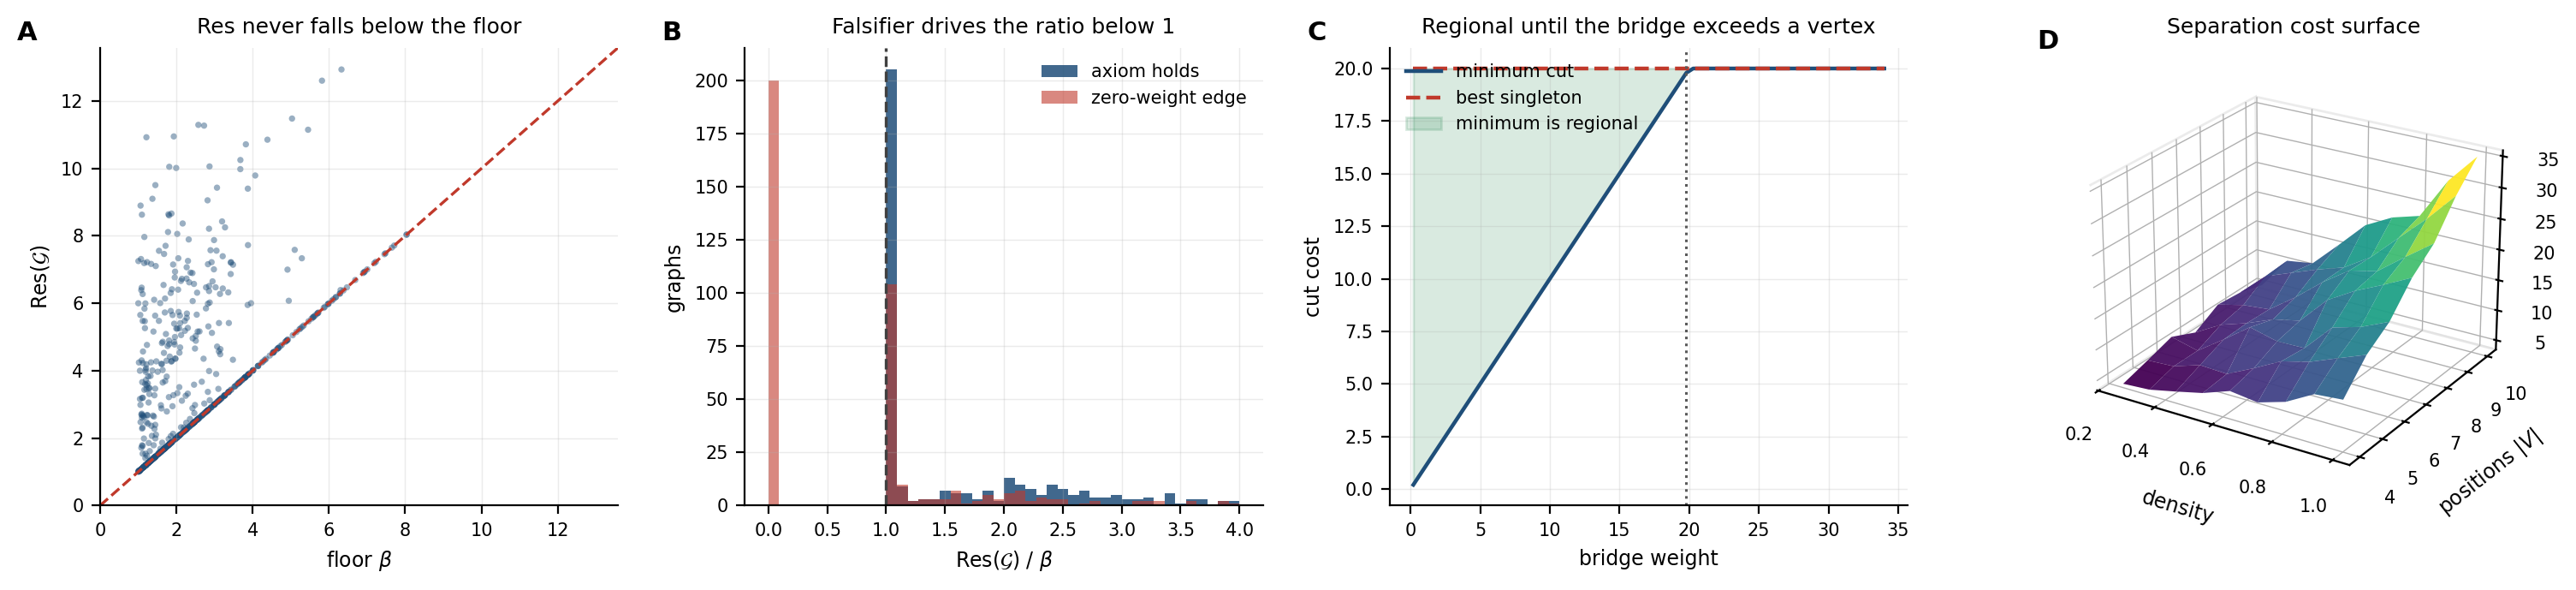
\includegraphics[width=\textwidth]{figures/panel_1}
    \caption{\textbf{Separation is bounded away from zero, and the bound is
    attained by a region rather than by a position.}
    (\textbf{A})~Separation cost $\Res(\Gph)$ on the linear $y$-axis
    ($1.01$ to $12.9$) versus the floor $\flo$ on the linear $x$-axis
    ($1.00$ to $8.04$), for $600$ randomly generated connected contact graphs
    on three to eight positions; the dashed line is the identity. Every point
    lies on or above it, so no graph separates a nonempty proper part from its
    complement more cheaply than its least edge weight. Points on the line are
    graphs whose minimum cut is a single cheapest edge; points above it are
    graphs in which every separation severs more
    (\Cref{thm:floor}).
    (\textbf{B})~Distribution of the ratio $\Res(\Gph)/\flo$ on the linear
    $x$-axis ($0$ to $4$) over $400$ graphs, with \Cref{ax:costly} holding
    (dark) and with one edge weight set to zero (light); the dashed line marks
    unity. The intact series lies entirely at or above $1$; the falsified
    series places $109$ of $200$ graphs at $0$. The bound is therefore a
    consequence of the axiom and not of the definition, since removing the
    axiom removes the bound.
    (\textbf{C})~Cut cost on the linear $y$-axis ($0$ to $20$) versus the
    weight of the joining edge on the linear $x$-axis ($0.2$ to $34$), for the
    two-triangle witness of \Cref{thm:regional} with all six internal weights
    fixed at $10$. The minimum cut (solid) rises with the bridge while the
    best singleton cut (dashed) is constant at $20$; the shaded interval is
    where the minimum is attained by a three-position region and by no
    singleton, and the dotted line marks the crossover at bridge weight $20$
    beyond which the two coincide. Individuation has extent
    (\Cref{cor:no-point}).
    (\textbf{D})~Three-dimensional surface of mean separation cost on the
    $z$-axis ($4.08$ to $35.3$) over edge density on the $x$-axis ($0.25$ to
    $1.0$) and position count $|\V|$ on the $y$-axis ($4$ to $10$), each cell
    the mean of $14$ graphs. The surface is strictly positive at every
    combination and rises with both parameters; there is no direction in the
    parameter space along which separation cost approaches zero, which is the
    absence of the limiting process that \Cref{rem:floor-content} identifies
    as the theorem's content. Viewing angle: elevation $24^{\circ}$, azimuth
    $-58^{\circ}$.}
    \label{fig:panel1}
\end{figure*}

\begin{figure*}[!htbp]
    \centering
    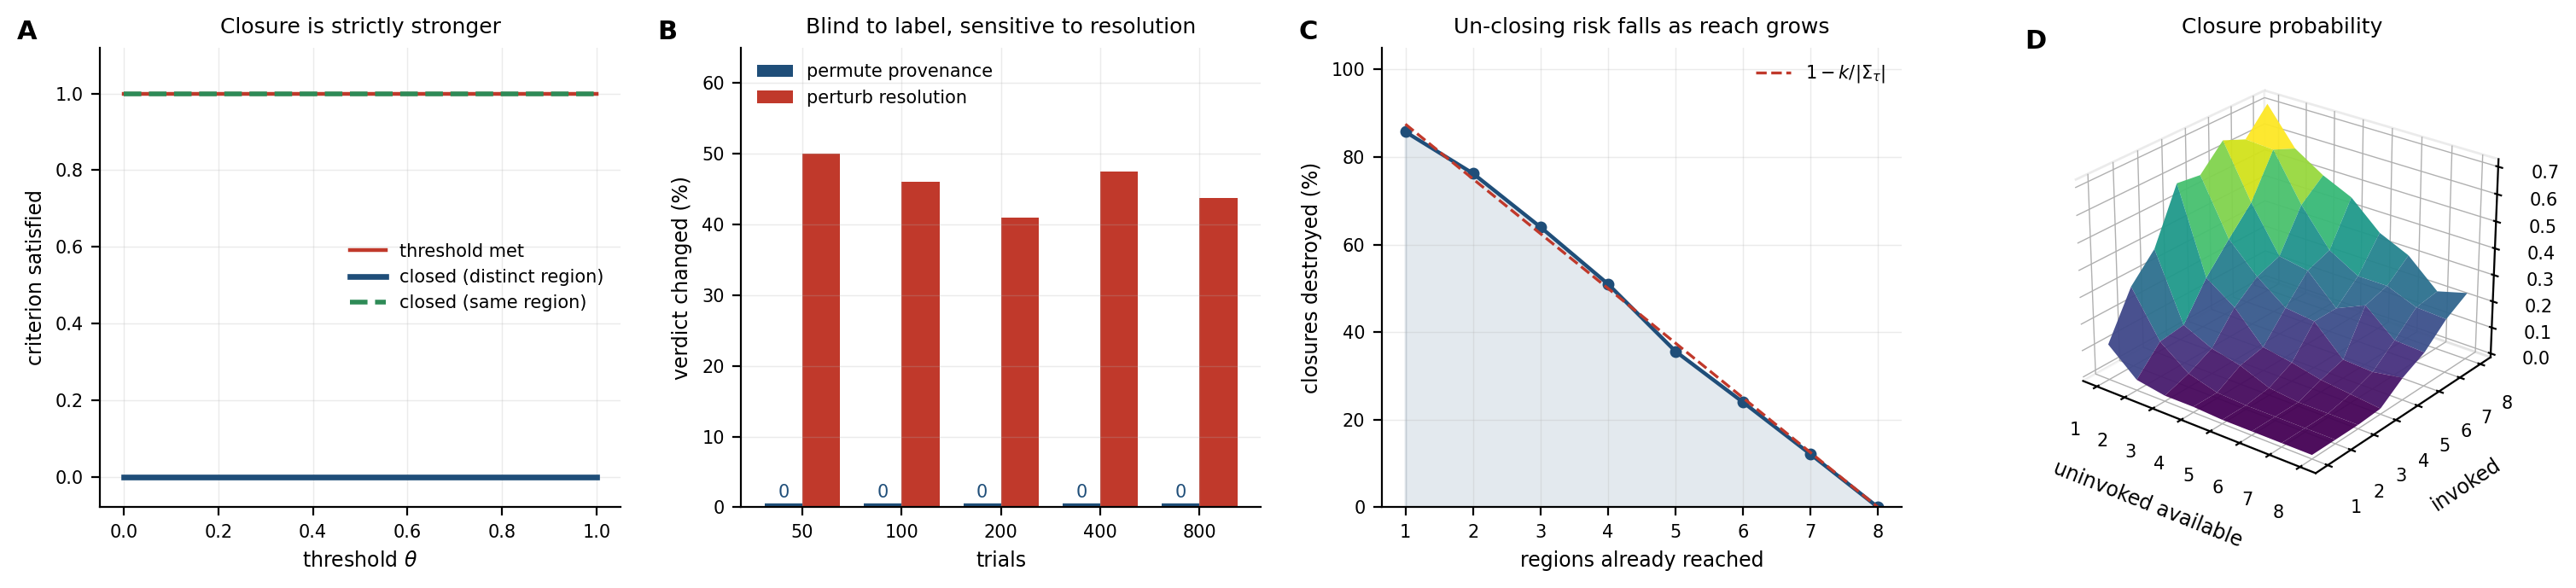
\includegraphics[width=\textwidth]{figures/panel_2}
    \caption{\textbf{Closure is not a threshold, does not read provenance, and
    is not monotone in what is available.}
    (\textbf{A})~Criterion satisfied, on the binary $y$-axis, versus the
    confidence threshold $\theta$ on the linear $x$-axis ($0$ to $1$), on the
    witness of \Cref{thm:closure-stronger}: two disjoint triangles joined by a
    single edge, with both considerations carrying confidence $1$. The
    threshold criterion (upper trace) is met at every $\theta$; the closure
    criterion (lower trace) fails at every $\theta$, because the uninvoked
    consideration resolves into the second triangle. Replacing that
    consideration by one resolving into the \emph{first} triangle restores
    closure at every $\theta$ (dashed, coincident with the upper trace),
    locating the failure in the distinct region rather than in the form of
    \Cref{def:closure}. No adjustment of $\theta$ converts one criterion into
    the other.
    (\textbf{B})~Percentage of verdicts changed on the linear $y$-axis versus
    the number of randomised configurations on the categorical $x$-axis ($50$
    to $800$). Permuting provenance labels changes the verdict in exactly
    zero cases at every sample size (dark, annotated, drawn as a rule at the
    axis since the bars have no height); perturbing \emph{resolutions} with
    the same machinery changes it in $41.0$ to $50.0$ per cent of cases
    (light). It is the asymmetry between the two counts, not the invariance
    alone, that distinguishes \Cref{thm:blind} from a definition too coarse to
    register anything: a definition insensitive to everything would have
    produced invariance under both perturbations.
    (\textbf{C})~Percentage of existing closures destroyed by adjoining one
    further available consideration, on the linear $y$-axis ($0$ to $85.8$),
    versus the number of regions the invoked set already reaches, on the
    linear $x$-axis ($1$ to $8$), drawn from a pool of eight distinct regions;
    the dashed line is the analytic prediction $1-k/|\Sig_\tau|$. The measured
    curve tracks it across the range and reaches zero exactly when the invoked
    reach exhausts the pool. A commitment can therefore lapse because
    something new became available, with no agent having changed its mind
    about anything already considered (\Cref{rem:not-mono-avail}).
    (\textbf{D})~Three-dimensional surface of the probability that a search is
    closed, on the $z$-axis ($0$ to $0.713$), over the number of uninvoked
    available considerations on the $x$-axis ($1$ to $8$) and the number
    invoked on the $y$-axis ($1$ to $8$), each cell $160$ draws from a
    six-region pool. The surface falls steeply along the availability axis and
    rises along the invoked axis: closure is a joint condition on both, and in
    particular is not a property of the evidence in hand
    (\Cref{prop:mono-invoked}). Viewing angle: elevation $26^{\circ}$, azimuth
    $-52^{\circ}$.}
    \label{fig:panel2}
\end{figure*}

\begin{figure*}[!htbp]
    \centering
    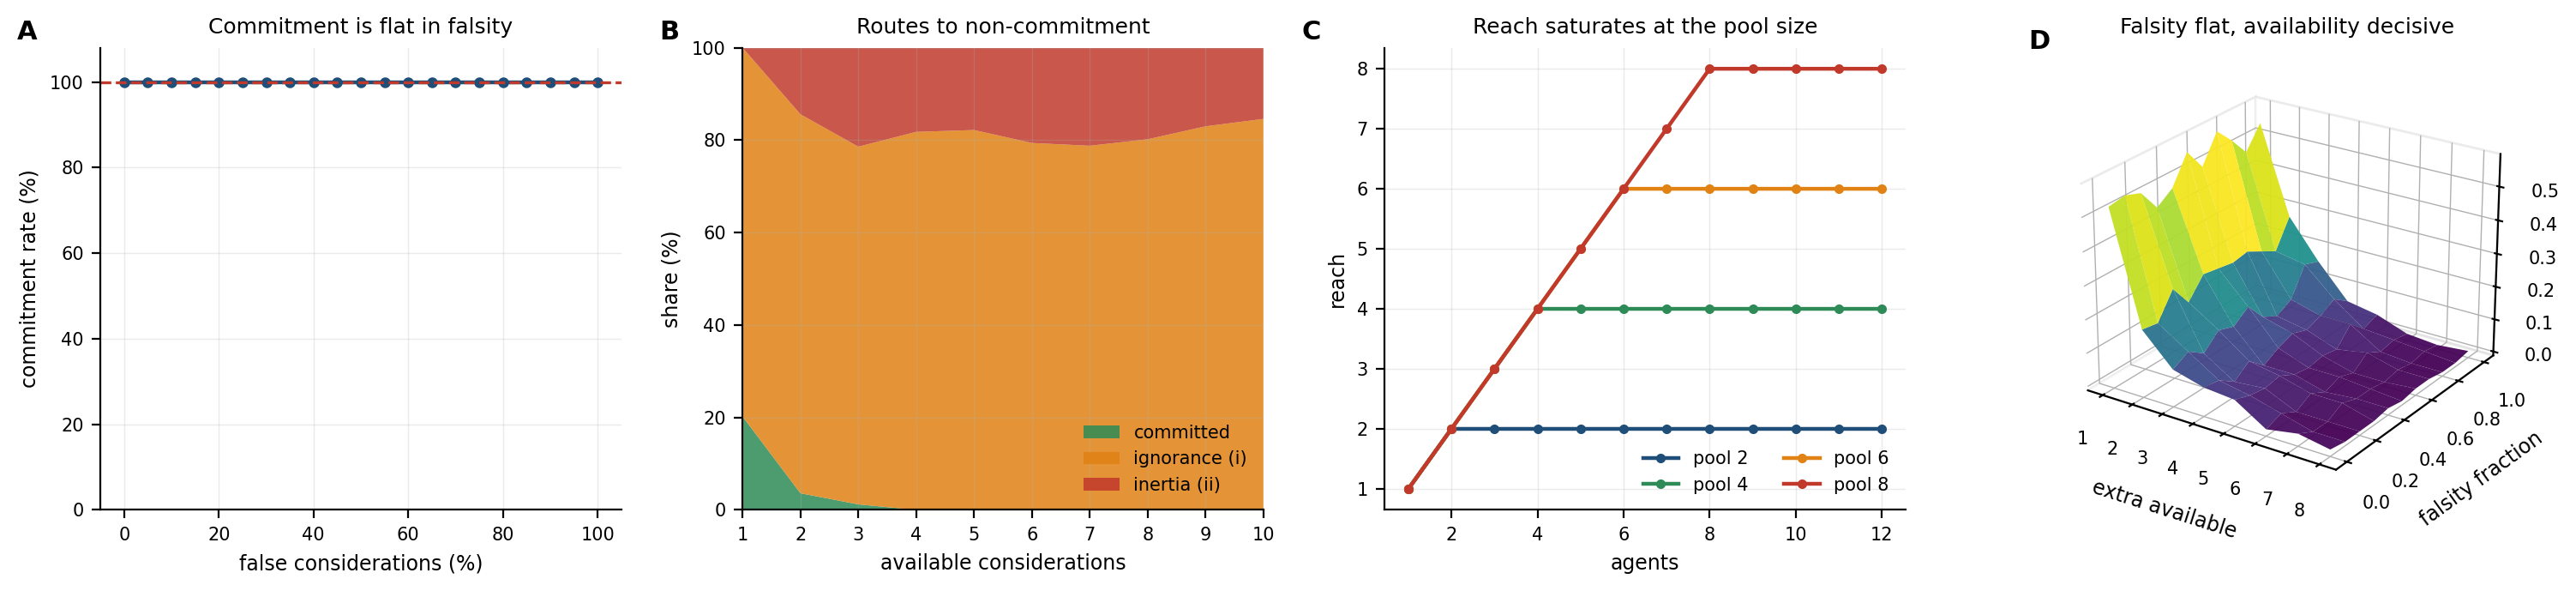
\includegraphics[width=\textwidth]{figures/panel_3}
    \caption{\textbf{Correctness is not a term in the commitment condition,
    and non-commitment decomposes into three structurally distinct routes.}
    (\textbf{A})~Commitment rate on the linear $y$-axis ($0$ to $108$ per
    cent) versus the percentage of considerations that are false on the linear
    $x$-axis ($0$ to $100$), holding resolutions fixed, $500$ configurations
    per point; the dashed line marks $100$ per cent. The measured rate is
    exactly $100$ per cent at every level of falsity including the endpoint at
    which \emph{every} consideration is false. Commitment is therefore
    invariant under substitution of false considerations for true ones with
    the same resolution (\Cref{thm:truth-blind}). The theorem does not assert
    that falsity is harmless: a population committed to the wrong region
    encounters the consequences of being there, but by the ordinary route of
    occupying an unsuitable region rather than through any failure of the
    mechanism (\Cref{rem:truth-scope}).
    (\textbf{B})~Share of outcomes on the linear $y$-axis ($0$ to $100$ per
    cent) versus the number of available considerations on the linear $x$-axis
    ($1$ to $10$), $500$ configurations per point, stacked by the
    classification of \Cref{prop:three-routes}. Commitment falls from $20.2$
    per cent at a single available consideration to below $1$ per cent by
    four; ignorance --- no invoked consideration reaches the target ---
    dominates throughout at $77$ to $82$ per cent; inertia --- the target is
    reached but closure fails --- grows as the available set does. The three
    are distinguished by different tests, which is why they present
    differently from the inside (\Cref{rem:three-feel}).
    (\textbf{C})~Reach on the linear $y$-axis ($1$ to $8$) versus population
    on the linear $x$-axis ($1$ to $12$), for pools of two, four, six and
    eight distinct resolutions. Each series grows one-for-one until the pool
    is exhausted and is exactly flat thereafter. Reach is bounded by the
    number of \emph{distinct} resolutions and not by headcount, and the
    ceiling $|\Sig_\tau(\Gph)|$ counts regions the graph possesses, so no
    recruitment raises it (\Cref{prop:ceiling,rem:heterogeneity}).
    (\textbf{D})~Three-dimensional surface of commitment probability on the
    $z$-axis ($0$ to $0.583$) over the number of extra available
    considerations on the $x$-axis ($1$ to $8$) and the falsity fraction on
    the $y$-axis ($0$ to $1$), $120$ draws per cell. The surface is flat along
    the falsity axis and falls sharply along the availability axis, exhibiting
    \Cref{thm:truth-blind} and \Cref{rem:not-mono-avail} on one pair of
    coordinates: what an agent believes wrongly does not move the verdict, and
    what it has not yet considered does. Viewing angle: elevation
    $24^{\circ}$, azimuth $-56^{\circ}$.}
    \label{fig:panel3}
\end{figure*}

\begin{figure*}[!htbp]
    \centering
    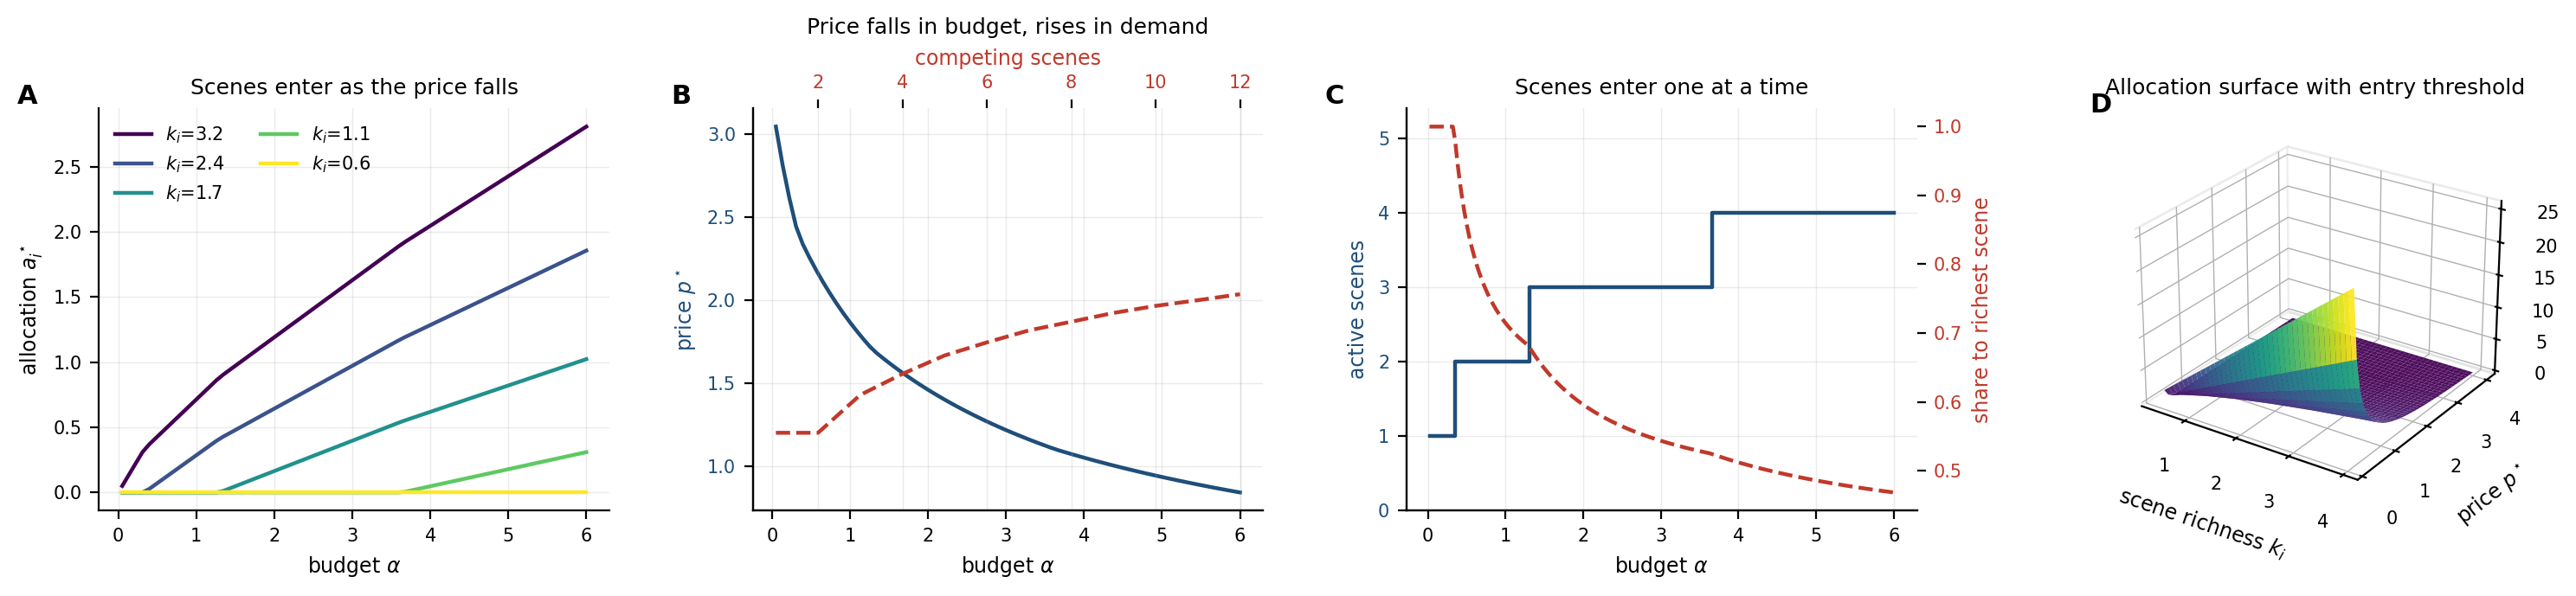
\includegraphics[width=\textwidth]{figures/panel_4}
    \caption{\textbf{A bounded capacity divides across concurrent demands by
    water-filling at a single price, with scenes entering at their own
    thresholds.}
    (\textbf{A})~Optimal allocation $a_i^{\star}$ on the linear $y$-axis ($0$
    to $2.81$) versus the budget $\att$ on the linear $x$-axis ($0.05$ to
    $6$), for five scenes with gain profiles $\gamma_i(a)=k_i\log(1+a)$ and
    richness $k_i\in\{3.2,2.4,1.7,1.1,0.6\}$. Each curve leaves zero at its
    own entry threshold --- the budget at which the price falls to
    $\gamma_i'(0)=k_i$ --- and the poorest scene remains unattended over the
    entire range plotted. Just above its threshold a scene receives a positive
    but arbitrarily small allocation, which is the formal minimal
    acknowledgement of \Cref{cor:token}.
    (\textbf{B})~Attention price $\price$ on the linear $y$-axis ($0.84$ to
    $3.05$) versus the budget on the lower linear $x$-axis ($0.05$ to $6$,
    solid) and versus the number of competing scenes on the upper linear
    $x$-axis ($1$ to $12$, dashed, $\price$ from $1.20$ to $2.04$). The price
    is monotone decreasing in capacity and monotone increasing in demand,
    both as \Cref{thm:waterfill} requires of the multiplier of a binding
    budget constraint.
    (\textbf{C})~Number of attended scenes on the left linear $y$-axis ($0$ to
    $5$, step) and the share of capacity received by the richest scene on the
    right linear $y$-axis ($0.5$ to $1.0$, dashed), versus the budget on the
    linear $x$-axis ($0.02$ to $6$). Scenes are taken up one at a time as the
    price crosses successive thresholds, while the richest scene's share falls
    monotonically from unity: the agent becomes thinly present in several
    contexts rather than fully present in one. This is the derived content of
    \Cref{cor:preoccupied}, and it is the one result in the figure conditional
    on the environmental assumption \Cref{ax:concave}; under increasing
    returns the optimum is concentration instead (\Cref{rem:nonconcave}).
    (\textbf{D})~Three-dimensional surface of the allocation
    $(\gamma_i')^{-1}(\price)=k_i/\price-1$ on the $z$-axis ($0$ to $25$) over
    scene richness $k_i$ on the $x$-axis ($0.4$ to $4.0$) and price $\price$
    on the $y$-axis ($0.15$ to $4.0$), clipped at zero where $k_i\le\price$.
    The ridge along which the surface leaves the zero plane is the entry
    threshold, and the divergence at small price is the regime in which an
    idle agent is forthcoming everywhere at once. Viewing angle: elevation
    $26^{\circ}$, azimuth $-56^{\circ}$.}
    \label{fig:panel4}
\end{figure*}

\begin{figure*}[!htbp]
    \centering
    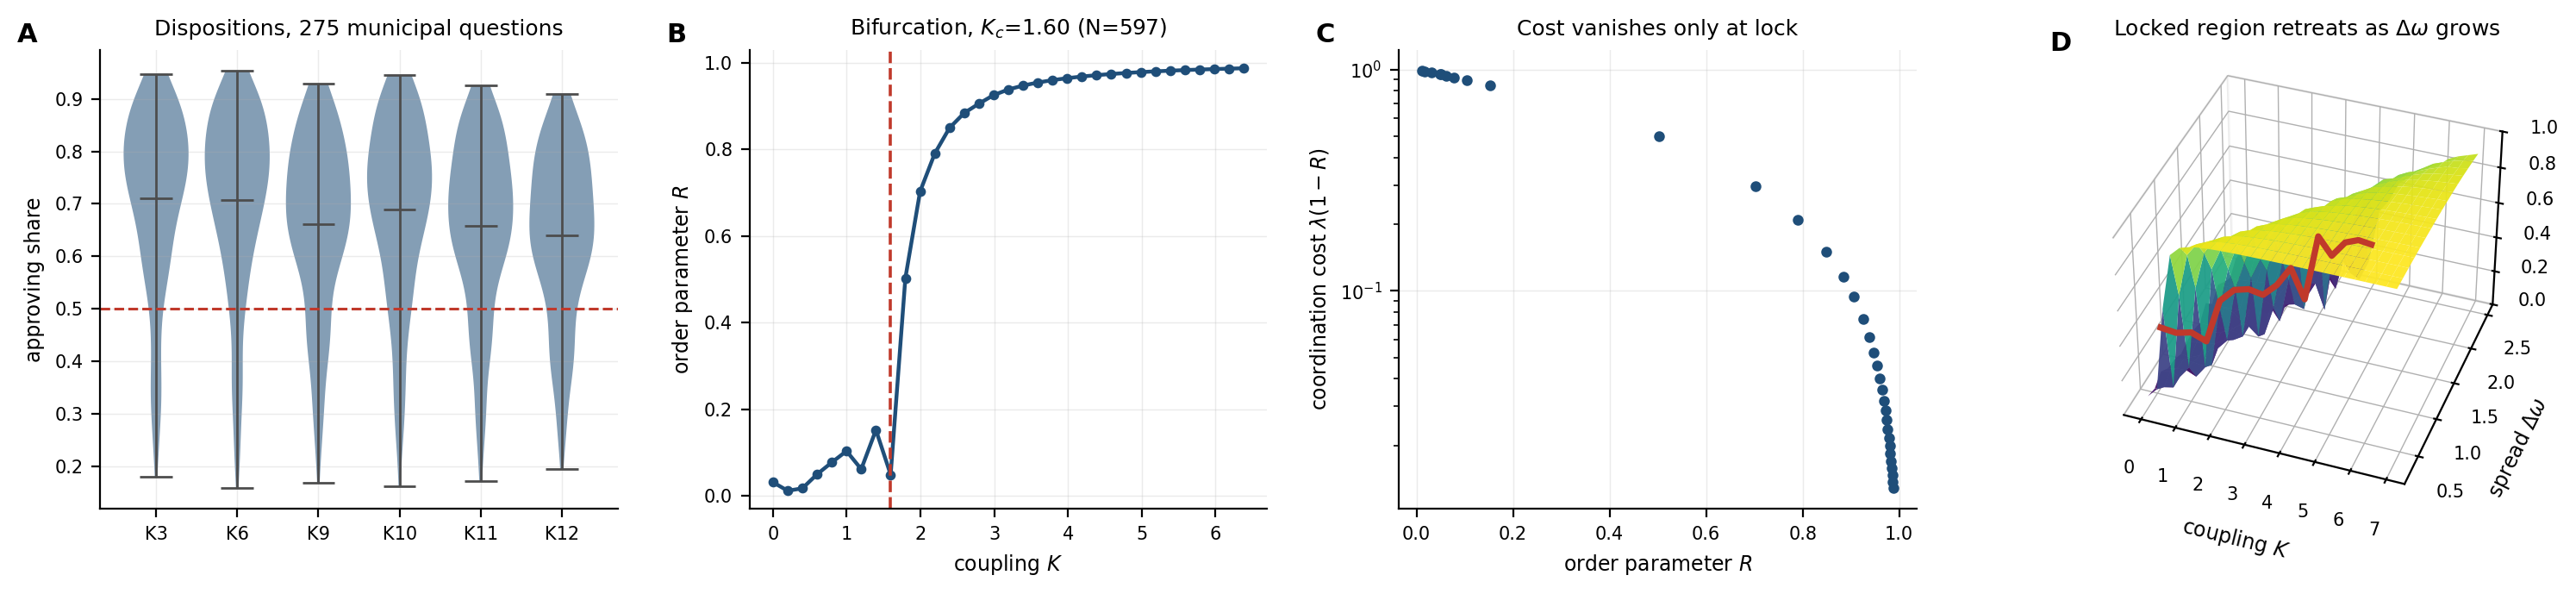
\includegraphics[width=\textwidth]{figures/panel_5}
    \caption{\textbf{The synchronisation threshold, measured on the
    heterogeneity of the Z\"urich record.}
    (\textbf{A})~Approving share on the linear $y$-axis ($0.158$ to $0.954$)
    for each of the six consistently reported municipal units on the
    categorical $x$-axis, as violin densities over all $275$ city questions of
    2002--2026 \citep{ssz_abstimmungen}; the dashed line marks the $0.5$
    majority. The dispersion between units, not their central tendency, is the
    velocity spread $\Delta\omega$ that fixes the threshold in the remaining
    charts, so the parameter is measured from the record rather than assumed.
    (\textbf{B})~Order parameter $\Ord$ on the linear $y$-axis ($0.012$ to
    $0.987$) versus coupling $K$ on the linear $x$-axis ($0$ to $6.38$), with
    each unit treated as a tempo class populated in proportion to its resident
    count, giving $N=597$ oscillators, integrated $3000$ steps at $dt=0.05$;
    the dashed line is the predicted critical coupling $\Kc=1.60$. Below it
    the order parameter remains at or under $0.107$ and does not drift upward
    under continued integration; above $2\Kc$ it exceeds $0.951$. The
    populating step is necessary rather than cosmetic: \Cref{thm:kuramoto}(ii)
    is a mean-field statement and six oscillators alone leave the transition
    buried in finite-size fluctuation.
    (\textbf{C})~Coordination cost $\lambda_c(1-\Ord)$ on the logarithmic
    $y$-axis ($0.0128$ to $0.988$) versus the order parameter on the linear
    $x$-axis ($0$ to $1$), evaluated on the achieved $\Ord$ of chart~B. The
    cost falls by nearly two decades only as $\Ord$ approaches unity and
    vanishes exactly at lock, which is the equality case of
    \Cref{thm:phaselock}; away from lock it is strictly positive.
    (\textbf{D})~Three-dimensional surface of the order parameter on the
    $z$-axis ($0$ to $1$) over coupling $K$ on the $x$-axis ($0$ to $7$) and
    velocity spread $\Delta\omega$ on the $y$-axis ($0.3$ to $2.5$), computed
    on one fixed standardised velocity sample of $400$ oscillators rescaled
    per row so that rows differ only in spread and not in sampling noise; the
    solid line is the predicted $\Kc=2\sigma_\omega\sqrt{2\pi}/\pi$ lifted onto
    the surface. The locked plateau retreats toward larger $K$ as
    heterogeneity grows, and the predicted threshold tracks the boundary. The
    residual roughness below the threshold is genuine finite-size fluctuation
    of $\Ord$ in the incoherent regime, not numerical noise, and is left
    unsmoothed. Viewing angle: elevation $38^{\circ}$, azimuth $-70^{\circ}$.}
    \label{fig:panel5}
\end{figure*}

\begin{figure*}[!htbp]
    \centering
    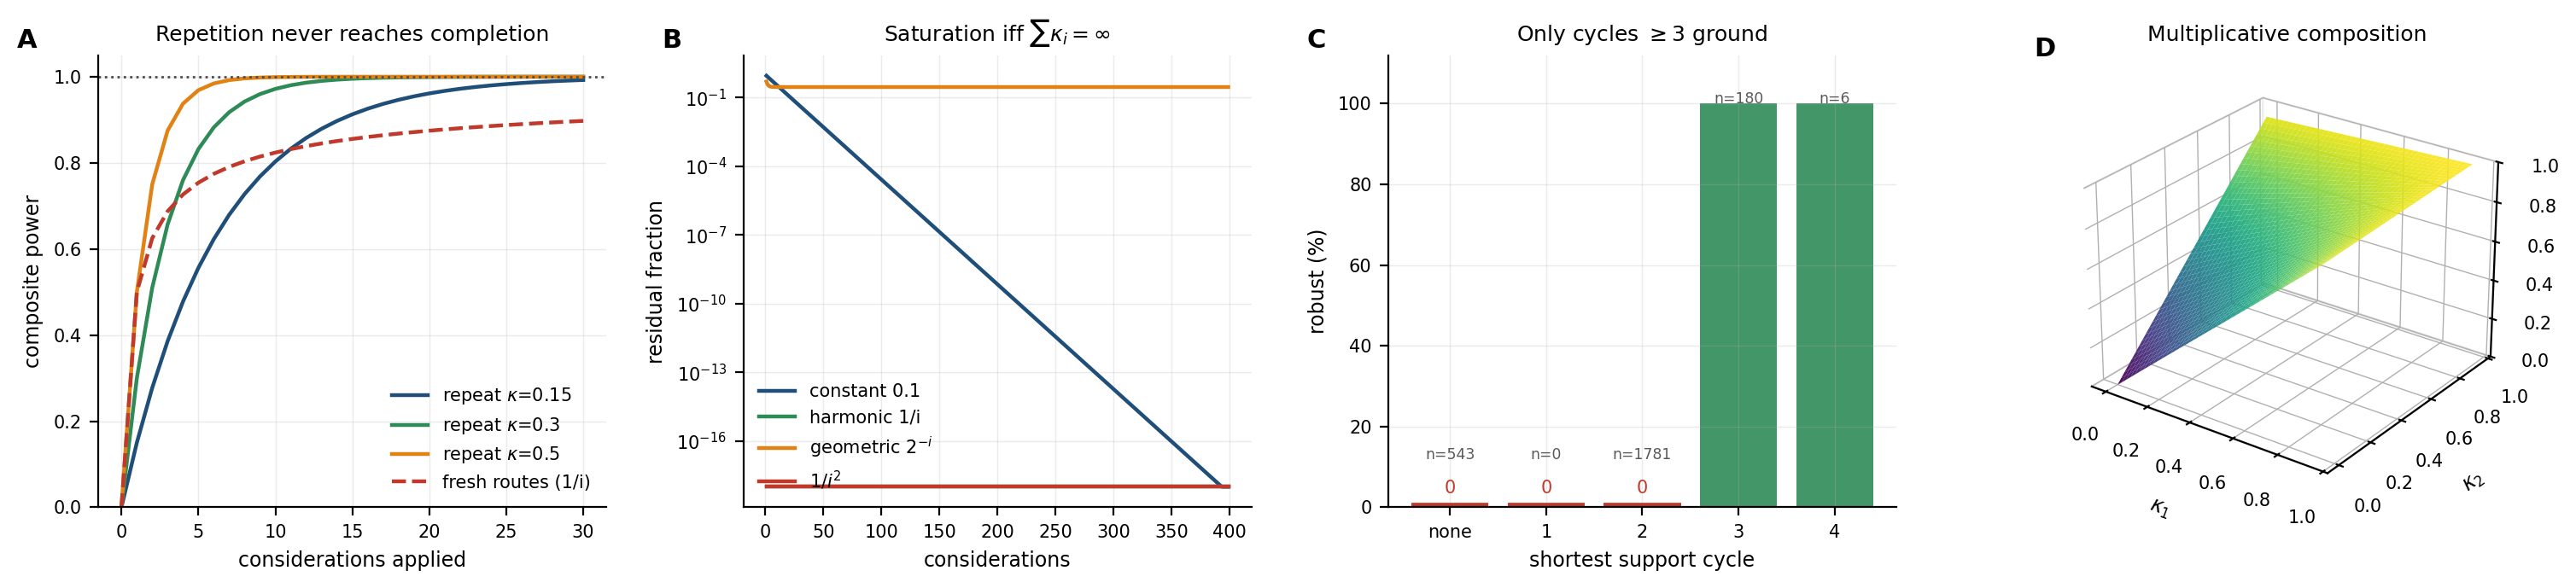
\includegraphics[width=\textwidth]{figures/panel_6}
    \caption{\textbf{Considerations compose multiplicatively, repetition
    saturates strictly below completion, and grounding requires a support
    cycle of length at least three.}
    (\textbf{A})~Composite power on the linear $y$-axis ($0$ to $1$) versus
    the number of considerations applied on the linear $x$-axis ($0$ to $30$),
    for a single consideration of power $\kappa\in\{0.15,0.30,0.50\}$ repeated
    (solid) and for a sequence of fresh routes with powers $0.5/i$ (dashed,
    reaching $0.897$ at $30$); the dotted line marks unity. Every repetition
    series increases, converges toward unity and attains it at no finite
    count, with strictly decaying increments
    (\Cref{cor:diminishing,cor:saturate}).
    (\textbf{B})~Residual fraction $\prod_i(1-\kappa_i)$ on the logarithmic
    $y$-axis ($10^{-18}$ to $1$) versus the number of considerations on the
    linear $x$-axis ($1$ to $399$), for four power sequences. The
    divergent-sum sequences (constant $0.1$; harmonic $1/i$) drive the
    residual toward zero; the convergent-sum sequences (geometric $2^{-i}$;
    inverse-square $1/i^{2}$) plateau at a positive constant and remain there.
    This is the dichotomy of \Cref{thm:saturation} and the structural
    condition on a long campaign: a proposal whose reachable considerations
    have summable powers is never closed by persistence
    (\Cref{rem:campaign}).
    (\textbf{C})~Percentage of support structures that are robust on the
    linear $y$-axis ($0$ to $100$) by shortest directed cycle length on the
    categorical $x$-axis, exhaustively over four-position digraphs with at
    most six edges, with the number of structures in each class annotated.
    Acyclic structures and cycles of length one and two are robust in no case
    and are drawn as rules at the axis with their zero marked; every structure
    whose shortest cycle has length three or four is robust without exception.
    Two elements can only assert each other; three can check each other
    (\Cref{thm:linear,thm:three}), and a repeated single item is a one-cycle
    and therefore grounds nothing (\Cref{cor:repeat-nothing}).
    (\textbf{D})~Three-dimensional surface of the composite power
    $1-(1-\kappa_1)(1-\kappa_2)$ on the $z$-axis ($0$ to $1$) over the two
    constituent powers on the $x$- and $y$-axes ($0$ to $0.95$). The sheet
    rises toward but never attains unity, and its curvature is the diminishing
    return each additional consideration closes of the remaining above-floor
    distance (\Cref{thm:multiplicative}). Viewing angle: elevation
    $26^{\circ}$, azimuth $-54^{\circ}$.}
    \label{fig:panel6}
\end{figure*}

\begin{figure*}[!htbp]
    \centering
    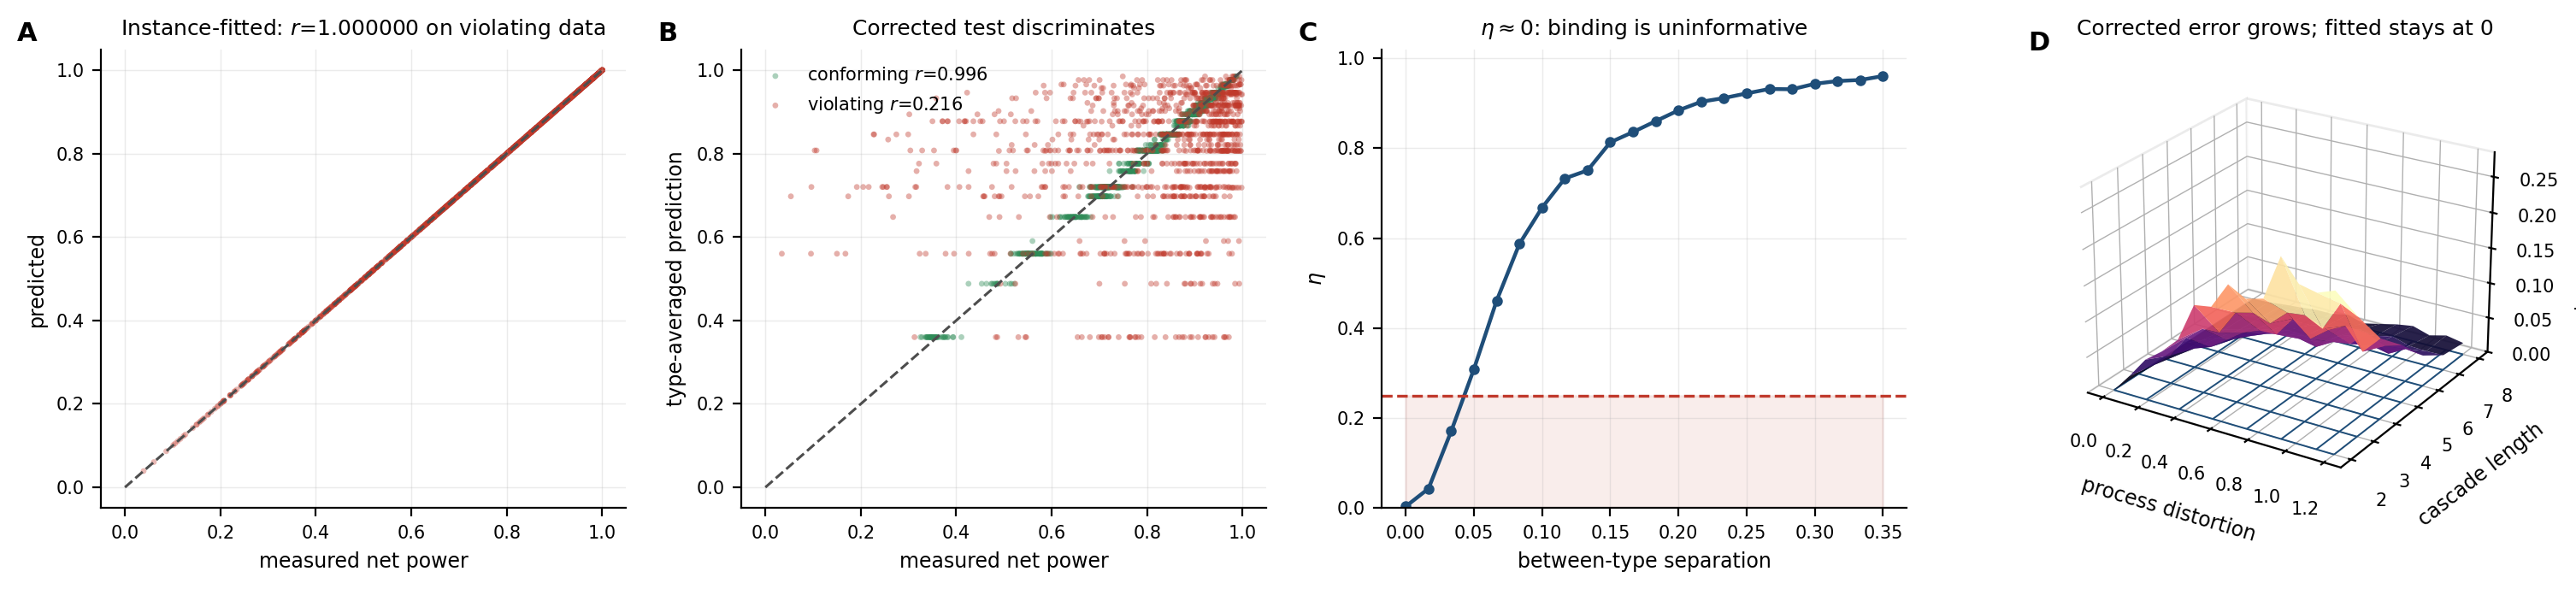
\includegraphics[width=\textwidth]{figures/panel_7}
    \caption{\textbf{The natural test of the composition law has no null; the
    type-averaged test does; and the diagnostic says when even it has no
    power.}
    (\textbf{A})~Instance-specific prediction $1-\prod_i(1-\kappa_i)$ on the
    linear $y$-axis ($0$ to $1$) versus the measured net power
    $(S_1-S_{n+1})/(S_1-\flo)$ on the linear $x$-axis ($0$ to $1$), for
    $1500$ cascades of length two to six generated by a process that violates
    \Cref{thm:multiplicative} by construction, each step's reduction being
    scaled by an arbitrary distortion factor. The points lie on the diagonal
    (dashed) with Pearson $r=1.000000$: under instance-specific estimation the
    two quantities are the \emph{same algebraic expression}, so the statistic
    attains its degenerate value on every data set whatsoever, including data
    generated by a process violating the law it purports to confirm. The test
    cannot fail and therefore has no power against any alternative
    (\Cref{thm:telescoping,cor:no-null}).
    (\textbf{B})~The same comparison under type-averaged estimation, in which
    the constituent powers are the means of their event types computed
    excluding the predicted cascade. Conforming data attain $r=0.996$ and
    data violating the composition law fall to $r=0.216$, with the violating
    cloud departing visibly from the diagonal. Breaking the dependence of the
    prediction on the predicted cascade's own observations restores a null
    (\Cref{thm:typeavg}).
    (\textbf{C})~Separation diagnostic $\eta=\Var_{\mathrm{b}}/
    (\Var_{\mathrm{b}}+\Var_{\mathrm{w}})$ on the linear $y$-axis ($0.004$ to
    $0.961$) versus the imposed between-type separation on the linear $x$-axis
    ($0$ to $0.35$), at fixed within-type dispersion; the shaded band below
    the dashed line at $0.25$ is the regime in which per-type means are
    indistinguishable. There, predictions are constant at fixed cascade length
    and no comparison among composition rules can be separated, so a negative
    result is evidence about the observable rather than about the process
    (\Cref{prop:uninformative}).
    (\textbf{D})~Three-dimensional mean absolute prediction error on the
    $z$-axis over process distortion on the $x$-axis ($0$ to $1.2$) and
    cascade length on the $y$-axis ($2$ to $8$), $60$ cascades per cell, for
    the type-averaged test (surface, rising to $0.247$) and the
    instance-specific test (wireframe, bounded by $5.7\times10^{-17}$ across
    the whole grid). The corrected error grows with distortion while the
    fitted error is pinned at floating-point zero for every process: the
    obstruction and its remedy in one view. Viewing angle: elevation
    $24^{\circ}$, azimuth $-58^{\circ}$.}
    \label{fig:panel7}
\end{figure*}

\begin{figure*}[!htbp]
    \centering
    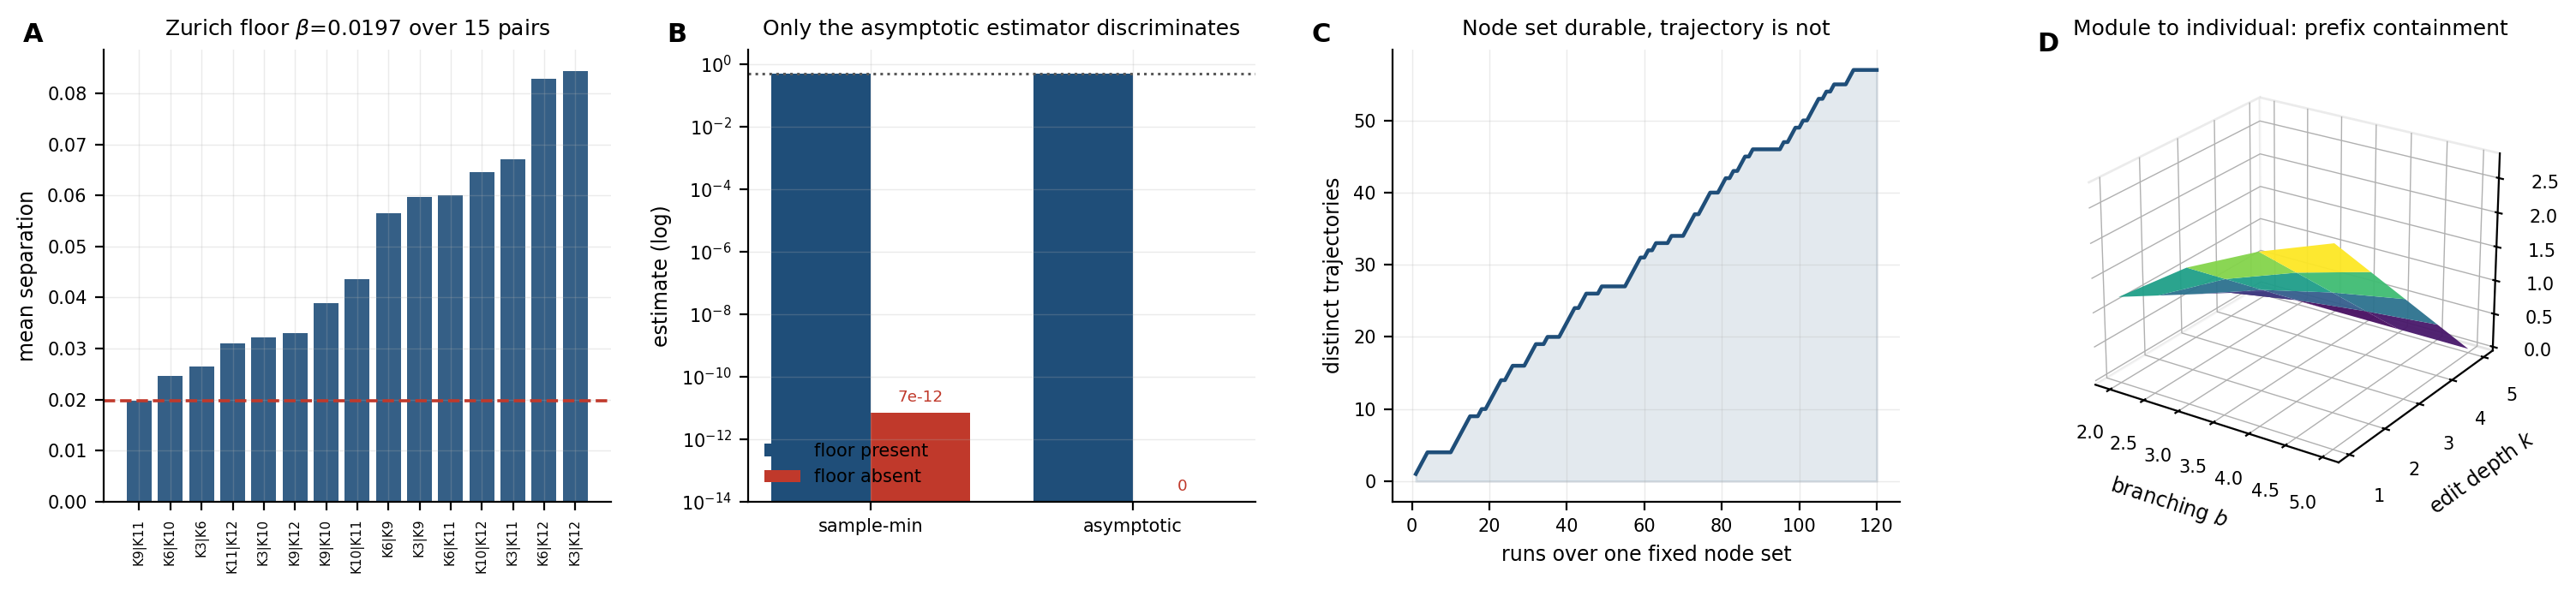
\includegraphics[width=\textwidth]{figures/panel_8}
    \caption{\textbf{The measured floor of the Z\"urich binding, the two
    discharges of the floor obligation, and the runtime's two durabilities.}
    (\textbf{A})~Mean separation on the linear $y$-axis ($0.0197$ to $0.0844$)
    for each of the $15$ receiver pairs on the categorical $x$-axis, sorted
    ascending, computed as the mean absolute difference of approving shares
    over all $275$ questions; the dashed line marks the least pair separation,
    which is the measured floor $\flo=0.0197$. It is strictly positive: even
    the two most similar units differ by about two percentage points on
    average across the record, so the floor is measured rather than assumed.
    Published shares are rounded to $0.1$ percentage points and two units
    therefore coincide exactly on $30$ of $4125$ single questions
    ($0.73$ per cent); a floor defined per question would be zero for a
    reason having nothing to do with the polity, which is why obligation (S4)
    is discharged on receiver \emph{pairs} over the whole record, as
    \Cref{def:cut} requires.
    (\textbf{B})~Floor estimate on the logarithmic $y$-axis ($10^{-14}$ to
    $3$) for the two discharges on the categorical $x$-axis, evaluated on a
    synthetic process with a genuine floor at $0.5$ (dark) and on one
    constructed to have no floor (light), $4000$ observations each; the dotted
    line marks the true value $0.5$. The sample-minimum estimator returns
    $0.500$ and $7\times10^{-12}$ --- positive on \emph{both} processes, so a
    positivity claim from it carries no evidential weight; the asymptotic
    estimator returns $0.499$ and exactly $0$, discriminating between them and
    therefore capable of being wrong (\Cref{rem:floor-obligation}).
    (\textbf{C})~Cumulative count of distinct trajectories on the linear
    $y$-axis ($1$ to $57$) versus runs executed on the linear $x$-axis ($1$ to
    $120$), over one fixed six-node set. The node set is durable and can be
    catalogued, frozen and imported; the induced causal edge relation is
    constituted by the run and is not schedulable in advance, so
    reproducibility attaches to the protocol and its provenance rather than to
    the readings (\Cref{thm:emergence,cor:repro,rem:repro-meaning}).
    (\textbf{D})~Three-dimensional surface of the blast radius $b^{D-k}$ on
    the logarithmic $z$-axis ($10^{0}$ to $10^{2.6}$) over branching factor
    $b$ on the $x$-axis ($2$ to $5$) and edit depth $k$ on the $y$-axis ($1$
    to $5$), at fixed tree depth $D=5$. An edit at depth $k$ touches exactly
    the leaves beneath its length-$k$ prefix and nothing else, falling from an
    entire imported subtree to a single leaf. A module is a short prefix and
    an individual a full-depth address in one space, so producing an
    individual by pruning is descent in that space rather than a change of
    kind (\Cref{prop:prefix,cor:two-depths}). Viewing angle: elevation
    $24^{\circ}$, azimuth $-56^{\circ}$.}
    \label{fig:panel8}
\end{figure*}
